%%%%%%%%%%%%%%%%%%%%%%%%%%%%%%%%%%%%%%%%%%%%%%%%%%%%%%%%%%%%%%%%%%%%%%%%%%%%%%%%
% WeBWorK Online Homework Delivery System
% Copyright � 2000-2007 The WeBWorK Project, http://openwebwork.sf.net/
% $CVSHeader: webwork2/conf/snippets/hardcopyPreamble.tex,v 1.3 2005/09/17 20:12:01 gage Exp $
% 
% This program is free software; you can redistribute it and/or modify it under
% the terms of either: (a) the GNU General Public License as published by the
% Free Software Foundation; either version 2, or (at your option) any later
% version, or (b) the "Artistic License" which comes with this package.
% 
% This program is distributed in the hope that it will be useful, but WITHOUT
% ANY WARRANTY; without even the implied warranty of MERCHANTABILITY or FITNESS
% FOR A PARTICULAR PURPOSE.  See either the GNU General Public License or the
% Artistic License for more details.
%%%%%%%%%%%%%%%%%%%%%%%%%%%%%%%%%%%%%%%%%%%%%%%%%%%%%%%%%%%%%%%%%%%%%%%%%%%%%%%%

\batchmode
\documentclass[10pt,dvips]{amsart}
\usepackage{amsmath,amsfonts,amssymb,multicol,setspace}
\usepackage[pdftex]{graphicx}
\usepackage{epstopdf}  % allows use of eps files with pdftex
\usepackage{epsf}
\usepackage{epsfig}
\usepackage{pslatex}
\usepackage[utf8]{inputenc}
\pagestyle{plain}
\textheight 9in
\oddsidemargin = -0.42in
\evensidemargin = -0.42in
\textwidth= 7.28in
\columnsep = .25in
\columnseprule = .4pt
\def\endline{\bigskip\hrule width \hsize height 0.8pt }
\newcommand{\lt}{<}
\newcommand{\gt}{>}
\newcommand{\less}{<}
\newcommand{\grt}{>}

% BEGIN capa tex macros

\newcommand{\capa}{{\sl C\kern-.10em\raise-.00ex\hbox{\rm A}\kern-.22em%
{\sl P}\kern-.14em\kern-.01em{\rm A}}}
  
\newenvironment{choicelist}
{\begin{list}{}
	{\setlength{\rightmargin}{0in}\setlength{\leftmargin}{0.13in}
	\setlength{\topsep}{0.05in}\setlength{\itemsep}{0.022in}
	\setlength{\parsep}{0in}\setlength{\belowdisplayskip}{0.04in}
	\setlength{\abovedisplayskip}{0.05in}
	\setlength{\abovedisplayshortskip}{-0.04in}
	\setlength{\belowdisplayshortskip}{0.04in}}
	}
{\end{list}}

% END capa tex macros 

\begin{document}
\voffset=-0.8in
\newpage
{\textbf \Large Final Exam, version 4} \hfill CSE 103, Fall 2014
\\

\vspace{.25in}

Name: \underline{\hspace{3in}}
\\

ID: \underline{\hspace{3.2in}}
\\

\vspace{0.5in}

On your desk you should have only the exam paper, writing tools, and
the cheat-sheet. The cheat-sheet is one page handwritten on both sides.

The exams are color coded. Your exam should have different color 
than that of your neighbours to the left, right and in front.

There are 11 questions in this exam, totalling 125 points.  The final
score is determined by summing all the points and taking the min of
the sum and 100. For a final grade of A+ it is necessary (but not
sufficient) to get more than 100 points in the final. 

Be clear and concise. Write your answers {\bf in the space provided}
after each question. Whenever possible, {\bf write your answers
as expressions, not as numbers}. If an expression is reused
later in the problem, you are encouraged to assign it to a letter
variable and use the variable in the later expressions. For example,
suppose in the first part of the problem you find the answer to be
$C(52,5)$ and that in a later part the answer is $22/C(52,5)$. You can
define in the first part $a=C(52,5)$ and write the second expression
as $22/a$. This will save you time and space and is easier for us to
grade.

Do your work at the empty space. If your answer is incorrect, we will
look at your work and give you credit if you were going in the right direction.

\vspace{0.2in}

\begin{center}
\begin{tabular}{|c|l|} \hline
\hspace{1in} & \hspace{1in} \\
1 & 12pt. \\ 
&  \\ \hline
2 & 9pt. \\
&  \\ \hline
3 & 10pt. \\
&  \\ \hline
4 & 10pt.\\
&  \\ \hline
5 & 10pt.\\
&  \\ \hline
6 & 9pt.\\
&  \\ \hline
7 & 9pt.\\
&  \\ \hline
8 & 9pt.\\
&  \\ \hline
9 & 20pt. \\
& \\ \hline
10 & 11pt. \\
& \\ \hline
11 & 16pt. \\
& \\ \hline
\end{tabular}
\end{center}
\begin{center}Total 125\end{center}

\vspace{0.2in}

This exam was graded by:\\
\hspace{1cm}abalsubr@eng.ucsd.edu
\hspace{1cm}iawwal@eng.ucsd.edu
\hspace{1cm}sjrao@eng.ucsd.edu
\hspace{1cm}zzhai@ucsd.edu
\hspace{1cm}yfreund@eng.ucsd.edu


\pagebreak

\columnwidth=\linewidth


%%%%%%%%%%%%%%%%%%%%%%%%%%%%%%%%%%%%%%%%%%%%%%%%%%%%%%%%%%%%%%%%%%%%%%%%%%%%%%%%
% WeBWorK Online Homework Delivery System
% Copyright � 2000-2007 The WeBWorK Project, http://openwebwork.sf.net/
% $CVSHeader: webwork2/conf/snippets/hardcopyProblemDivider.tex,v 1.3 2004/06/24 21:10:50 dpvc Exp $
% 
% This program is free software; you can redistribute it and/or modify it under
% the terms of either: (a) the GNU General Public License as published by the
% Free Software Foundation; either version 2, or (at your option) any later
% version, or (b) the "Artistic License" which comes with this package.
% 
% This program is distributed in the hope that it will be useful, but WITHOUT
% ANY WARRANTY; without even the implied warranty of MERCHANTABILITY or FITNESS
% FOR A PARTICULAR PURPOSE.  See either the GNU General Public License or the
% Artistic License for more details.
%%%%%%%%%%%%%%%%%%%%%%%%%%%%%%%%%%%%%%%%%%%%%%%%%%%%%%%%%%%%%%%%%%%%%%%%%%%%%%%%



      \ifx\pgmlMarker\undefined
        \newdimen\pgmlMarker \pgmlMarker=0.00314159pt  % hack to lett if \newline was used
      \fi
      \ifx\oldnewline\undefined \let\oldnewline=\newline \fi
      \def\newline{\oldnewline\hskip-\pgmlMarker\hskip\pgmlMarker\relax}%
      \parindent=0pt
      \catcode`\^^M=\active
      \def^^M{\ifmmode\else\fi\ignorespaces}%  skip paragraph breaks in the preamble
      \def\par{\ifmmode\else\endgraf\fi\ignorespaces}%
    {\bf 1.} (12 pts) \ifdim\lastskip=\pgmlMarker
  \let\pgmlPar=\relax
 \else
  \let\pgmlPar=\par
  \vadjust{\kern3pt}%
\fi

%%%%%%%%%%%%%%%%%%%%%%%%%%%%%%%%%%%%%%
%
%    definitions for PGML
%

\ifx\pgmlCount\undefined  % don not redefine if multiple files load PGML.pl
  \newcount\pgmlCount
  \newdimen\pgmlPercent
  \newdimen\pgmlPixels  \pgmlPixels=.5pt
\fi
\pgmlPercent=.01\hsize

\def\pgmlSetup{%
  \parskip=10pt \parindent=0pt
%  \ifdim\lastskip=\pgmlMarker\else\par\fi
  \pgmlPar
}%

\def\pgmlIndent{\par\advance\leftskip by 2em \advance\pgmlPercent by .02em \pgmlCount=0}%
\def\pgmlbulletItem{\par\indent\llap{$\bullet$ }\ignorespaces}%
\def\pgmlcircleItem{\par\indent\llap{$\circ$ }\ignorespaces}%
\def\pgmlsquareItem{\par\indent\llap{\vrule height 1ex width .75ex depth -.25ex\ }\ignorespaces}%
\def\pgmlnumericItem{\par\indent\advance\pgmlCount by 1 \llap{\the\pgmlCount. }\ignorespaces}%
\def\pgmlalphaItem{\par\indent{\advance\pgmlCount by `\a \llap{\char\pgmlCount. }}\advance\pgmlCount by 1\ignorespaces}%
\def\pgmlAlphaItem{\par\indent{\advance\pgmlCount by `\A \llap{\char\pgmlCount. }}\advance\pgmlCount by 1\ignorespaces}%
\def\pgmlromanItem{\par\indent\advance\pgmlCount by 1 \llap{\romannumeral\pgmlCount. }\ignorespaces}%
\def\pgmlRomanItem{\par\indent\advance\pgmlCount by 1 \llap{\uppercase\expandafter{\romannumeral\pgmlCount}. }\ignorespaces}%

\def\pgmlCenter{%
  \par \parfillskip=0pt
  \advance\leftskip by 0pt plus .5\hsize
  \advance\rightskip by 0pt plus .5\hsize
  \def\pgmlBreak{\break}%
}%
\def\pgmlRight{%
  \par \parfillskip=0pt
  \advance\leftskip by 0pt plus \hsize
  \def\pgmlBreak{\break}%
}%

\def\pgmlBreak{\\}%

\def\pgmlHeading#1{%
  \par\bfseries
  \ifcase#1 \or\huge \or\LARGE \or\large \or\normalsize \or\footnotesize \or\scriptsize \fi
}%

\def\pgmlRule#1#2{%
  \par\noindent
  \hbox{%
    \strut%
    \dimen1=\ht\strutbox%
    \advance\dimen1 by -#2%
    \divide\dimen1 by 2%
    \advance\dimen2 by -\dp\strutbox%
    \raise\dimen1\hbox{\vrule width #1 height #2 depth 0pt}%
  }%
  \par
}%

\def\pgmlIC#1{\futurelet\pgmlNext\pgmlCheckIC}%
\def\pgmlCheckIC{\ifx\pgmlNext\pgmlSpace \/\fi}%
{\def\getSpace#1{\global\let\pgmlSpace= }\getSpace{} }%

{\catcode`\ =12\global\let\pgmlSpaceChar= }%
{\obeylines\gdef\pgmlPreformatted{\par\small\ttfamily\hsize=10\hsize\obeyspaces\obeylines\let^^M=\pgmlNL\pgmlNL}}%
\def\pgmlNL{\par\bgroup\catcode`\ =12\pgmlTestSpace}%
\def\pgmlTestSpace{\futurelet\next\pgmlTestChar}%
\def\pgmlTestChar{\ifx\next\pgmlSpaceChar\ \pgmlTestNext\fi\egroup}%
\def\pgmlTestNext\fi\egroup#1{\fi\pgmlTestSpace}%


%%%%%%%%%%%%%%%%%%%%%%%%%%%%%%%%%%%%%%
{\pgmlSetup
Let $X_1, X_2, \ldots, X_{100}$ be the outcomes of $100$ independent tosses of a fair coin.\pgmlBreak
$P(X_i=0)=P(X_i=1)=0.5$
\vskip\baselineskip
{\pgmlIndent\let\pgmlItem=\pgmlnumericItem


\pgmlItem{}(1 pt) $\mathbb{E}(X_1) = $\mbox{  \parbox[t]{20ex}{\hrulefill}  }



\pgmlItem{}(1 pt) $var(X_1) = $\mbox{  \parbox[t]{20ex}{\hrulefill}  }
\par}%
\vskip\baselineskip

\vskip\baselineskip
Define the random variable $X = X_1 - X_2$. 
{\pgmlIndent\let\pgmlItem=\pgmlnumericItem


\pgmlItem{}(1 pt) $\mathbb{E}(X) = $\mbox{  \parbox[t]{20ex}{\hrulefill}  }



\pgmlItem{}(1 pt) $var(X) = $\mbox{  \parbox[t]{20ex}{\hrulefill}  }
\par}%
\vskip\baselineskip

\vskip\baselineskip
Define the random variable $Y = X_1 - 2X_2 + X_3$. 
{\pgmlIndent\let\pgmlItem=\pgmlnumericItem


\pgmlItem{}(2 pts) $\mathbb{E}(Y) = $\mbox{  \parbox[t]{20ex}{\hrulefill}  }



\pgmlItem{}(2 pts) $var(Y) = $\mbox{  \parbox[t]{20ex}{\hrulefill}  }
\par}%
\vskip\baselineskip

\vskip\baselineskip
Define the random variable $Z = X_1 - X_2 + X_3 - X_4 + ... + X_{81} - X_{82}$. 
{\pgmlIndent\let\pgmlItem=\pgmlnumericItem


\pgmlItem{}(2 pts) $\mathbb{E}(Z) = $\mbox{  \parbox[t]{20ex}{\hrulefill}  }



\pgmlItem{}(2 pts) $var(Z) = $\mbox{  \parbox[t]{20ex}{\hrulefill}  }

\par}%
\par}%
%%%%%%%%%%%%%%%%%%%%%%%%%%%%%%%%%%%%%%%%%%%%%%%%%%%%%%%%%%%%%%%%%%%%%%%%%%%%%%%%
% WeBWorK Online Homework Delivery System
% Copyright � 2000-2007 The WeBWorK Project, http://openwebwork.sf.net/
% $CVSHeader: webwork2/conf/snippets/hardcopyProblemDivider.tex,v 1.3 2004/06/24 21:10:50 dpvc Exp $
% 
% This program is free software; you can redistribute it and/or modify it under
% the terms of either: (a) the GNU General Public License as published by the
% Free Software Foundation; either version 2, or (at your option) any later
% version, or (b) the "Artistic License" which comes with this package.
% 
% This program is distributed in the hope that it will be useful, but WITHOUT
% ANY WARRANTY; without even the implied warranty of MERCHANTABILITY or FITNESS
% FOR A PARTICULAR PURPOSE.  See either the GNU General Public License or the
% Artistic License for more details.
%%%%%%%%%%%%%%%%%%%%%%%%%%%%%%%%%%%%%%%%%%%%%%%%%%%%%%%%%%%%%%%%%%%%%%%%%%%%%%%%


\pagebreak{\bf 2.} (9 pts) \ifdim\lastskip=\pgmlMarker
  \let\pgmlPar=\relax
 \else
  \let\pgmlPar=\par
  \vadjust{\kern3pt}%
\fi

%%%%%%%%%%%%%%%%%%%%%%%%%%%%%%%%%%%%%%
%
%    definitions for PGML
%

\ifx\pgmlCount\undefined  % don not redefine if multiple files load PGML.pl
  \newcount\pgmlCount
  \newdimen\pgmlPercent
  \newdimen\pgmlPixels  \pgmlPixels=.5pt
\fi
\pgmlPercent=.01\hsize

\def\pgmlSetup{%
  \parskip=10pt \parindent=0pt
%  \ifdim\lastskip=\pgmlMarker\else\par\fi
  \pgmlPar
}%

\def\pgmlIndent{\par\advance\leftskip by 2em \advance\pgmlPercent by .02em \pgmlCount=0}%
\def\pgmlbulletItem{\par\indent\llap{$\bullet$ }\ignorespaces}%
\def\pgmlcircleItem{\par\indent\llap{$\circ$ }\ignorespaces}%
\def\pgmlsquareItem{\par\indent\llap{\vrule height 1ex width .75ex depth -.25ex\ }\ignorespaces}%
\def\pgmlnumericItem{\par\indent\advance\pgmlCount by 1 \llap{\the\pgmlCount. }\ignorespaces}%
\def\pgmlalphaItem{\par\indent{\advance\pgmlCount by `\a \llap{\char\pgmlCount. }}\advance\pgmlCount by 1\ignorespaces}%
\def\pgmlAlphaItem{\par\indent{\advance\pgmlCount by `\A \llap{\char\pgmlCount. }}\advance\pgmlCount by 1\ignorespaces}%
\def\pgmlromanItem{\par\indent\advance\pgmlCount by 1 \llap{\romannumeral\pgmlCount. }\ignorespaces}%
\def\pgmlRomanItem{\par\indent\advance\pgmlCount by 1 \llap{\uppercase\expandafter{\romannumeral\pgmlCount}. }\ignorespaces}%

\def\pgmlCenter{%
  \par \parfillskip=0pt
  \advance\leftskip by 0pt plus .5\hsize
  \advance\rightskip by 0pt plus .5\hsize
  \def\pgmlBreak{\break}%
}%
\def\pgmlRight{%
  \par \parfillskip=0pt
  \advance\leftskip by 0pt plus \hsize
  \def\pgmlBreak{\break}%
}%

\def\pgmlBreak{\\}%

\def\pgmlHeading#1{%
  \par\bfseries
  \ifcase#1 \or\huge \or\LARGE \or\large \or\normalsize \or\footnotesize \or\scriptsize \fi
}%

\def\pgmlRule#1#2{%
  \par\noindent
  \hbox{%
    \strut%
    \dimen1=\ht\strutbox%
    \advance\dimen1 by -#2%
    \divide\dimen1 by 2%
    \advance\dimen2 by -\dp\strutbox%
    \raise\dimen1\hbox{\vrule width #1 height #2 depth 0pt}%
  }%
  \par
}%

\def\pgmlIC#1{\futurelet\pgmlNext\pgmlCheckIC}%
\def\pgmlCheckIC{\ifx\pgmlNext\pgmlSpace \/\fi}%
{\def\getSpace#1{\global\let\pgmlSpace= }\getSpace{} }%

{\catcode`\ =12\global\let\pgmlSpaceChar= }%
{\obeylines\gdef\pgmlPreformatted{\par\small\ttfamily\hsize=10\hsize\obeyspaces\obeylines\let^^M=\pgmlNL\pgmlNL}}%
\def\pgmlNL{\par\bgroup\catcode`\ =12\pgmlTestSpace}%
\def\pgmlTestSpace{\futurelet\next\pgmlTestChar}%
\def\pgmlTestChar{\ifx\next\pgmlSpaceChar\ \pgmlTestNext\fi\egroup}%
\def\pgmlTestNext\fi\egroup#1{\fi\pgmlTestSpace}%


%%%%%%%%%%%%%%%%%%%%%%%%%%%%%%%%%%%%%%
{\pgmlSetup
For the following joint probability matrices, fill in the missing values and answer the questions. 
(``Correlated'' = either positively or negatively correlated.)
\par}%

\par\smallskip\begin{center}\begin{tabular}{|c|c|c|c|c|} \hline

 & X=1   &  X=2   & X=3  &Marginal over Y \\ \hline 

Y=1 & 1/10 & & &3/10 \\ \hline 

Y=2 & 1/5  &1/10 &0 &3/10 \\ \hline 

Y=3 &1/5 & 1/5 & 0  & 2/5  \\ \hline 

Marginal over X &   & 2/5  & 1/10  &* \\ \hline 


\end {tabular}\end{center}\par\smallskip


{\pgmlSetup
{\pgmlIndent\let\pgmlItem=\pgmlbulletItem


\pgmlItem{}(1pt)Are $X$ and $Y$ dependent? \mbox{  \parbox[t]{20ex}{\hrulefill}  }



\pgmlItem{}(1pt)Are $X$ and $Y$ correlated? \mbox{  \parbox[t]{20ex}{\hrulefill}  }

\par}%
\par}%
{\pgmlSetup
{\pgmlIndent\let\pgmlItem=\pgmlbulletItem


\pgmlItem{}(1pt)$P(Y=3|X=2) = $ \mbox{  \parbox[t]{20ex}{\hrulefill}  }


\par}%
\par}%

\par\smallskip\begin{center}\begin{tabular}{|c|c|c|c|c|} \hline

 & X=1   &  X=2   & X=3  &Marginal over Y \\ \hline 

Y=1 & 1/15 &1/15 &1/15 & \\ \hline 

Y=2 & 2/15  &2/15 &2/15 &2/5 \\ \hline 

Y=3 & & 2/15 &   & 2/5  \\ \hline 

Marginal over X & 1/3  & 1/3  & 1/3  &* \\ \hline 


\end {tabular}\end{center}\par\smallskip


{\pgmlSetup
{\pgmlIndent\let\pgmlItem=\pgmlbulletItem


\pgmlItem{}(1pt)Are $X$ and $Y$ dependent? \mbox{  \parbox[t]{20ex}{\hrulefill}  }



\pgmlItem{}(1pt)Are $X$ and $Y$ correlated? \mbox{  \parbox[t]{20ex}{\hrulefill}  }

\par}%
\par}%
{\pgmlSetup
{\pgmlIndent\let\pgmlItem=\pgmlbulletItem


\pgmlItem{}(1pt)$P(X=1|Y=2) = $ \mbox{  \parbox[t]{20ex}{\hrulefill}  }


\par}%
\par}%

\par\smallskip\begin{center}\begin{tabular}{|c|c|c|c|c|} \hline

 & X=1   &  X=2   & X=3  &Marginal over Y \\ \hline 

Y=1 & 1/8 &0 &1/8 &1/4 \\ \hline 

Y=2 & 0  &1/2 &0 & \\ \hline 

Y=3 &1/8 & 0 & 1/8  & 1/4  \\ \hline 

Marginal over X & 1/4  &   &   &* \\ \hline 


\end {tabular}\end{center}\par\smallskip


{\pgmlSetup
{\pgmlIndent\let\pgmlItem=\pgmlbulletItem


\pgmlItem{}(1pt)Are $X$ and $Y$ dependent? \mbox{  \parbox[t]{20ex}{\hrulefill}  }



\pgmlItem{}(1pt)Are $X$ and $Y$ correlated? \mbox{  \parbox[t]{20ex}{\hrulefill}  }

\par}%
\par}%
{\pgmlSetup
{\pgmlIndent\let\pgmlItem=\pgmlbulletItem


\pgmlItem{}(1pt)$P(Y=2|X=2) = $ \mbox{  \parbox[t]{20ex}{\hrulefill}  }


\par}%
\par}%
%%%%%%%%%%%%%%%%%%%%%%%%%%%%%%%%%%%%%%%%%%%%%%%%%%%%%%%%%%%%%%%%%%%%%%%%%%%%%%%%
% WeBWorK Online Homework Delivery System
% Copyright � 2000-2007 The WeBWorK Project, http://openwebwork.sf.net/
% $CVSHeader: webwork2/conf/snippets/hardcopyProblemDivider.tex,v 1.3 2004/06/24 21:10:50 dpvc Exp $
% 
% This program is free software; you can redistribute it and/or modify it under
% the terms of either: (a) the GNU General Public License as published by the
% Free Software Foundation; either version 2, or (at your option) any later
% version, or (b) the "Artistic License" which comes with this package.
% 
% This program is distributed in the hope that it will be useful, but WITHOUT
% ANY WARRANTY; without even the implied warranty of MERCHANTABILITY or FITNESS
% FOR A PARTICULAR PURPOSE.  See either the GNU General Public License or the
% Artistic License for more details.
%%%%%%%%%%%%%%%%%%%%%%%%%%%%%%%%%%%%%%%%%%%%%%%%%%%%%%%%%%%%%%%%%%%%%%%%%%%%%%%%



      \ifx\pgmlMarker\undefined
        \newdimen\pgmlMarker \pgmlMarker=0.00314159pt  % hack to lett if \newline was used
      \fi
      \ifx\oldnewline\undefined \let\oldnewline=\newline \fi
      \def\newline{\oldnewline\hskip-\pgmlMarker\hskip\pgmlMarker\relax}%
      \parindent=0pt
      \catcode`\^^M=\active
      \def^^M{\ifmmode\else\fi\ignorespaces}%  skip paragraph breaks in the preamble
      \def\par{\ifmmode\else\endgraf\fi\ignorespaces}%
    \pagebreak{\bf 3.} (10 pts) \ifdim\lastskip=\pgmlMarker
  \let\pgmlPar=\relax
 \else
  \let\pgmlPar=\par
  \vadjust{\kern3pt}%
\fi

%%%%%%%%%%%%%%%%%%%%%%%%%%%%%%%%%%%%%%
%
%    definitions for PGML
%

\ifx\pgmlCount\undefined  % don not redefine if multiple files load PGML.pl
  \newcount\pgmlCount
  \newdimen\pgmlPercent
  \newdimen\pgmlPixels  \pgmlPixels=.5pt
\fi
\pgmlPercent=.01\hsize

\def\pgmlSetup{%
  \parskip=10pt \parindent=0pt
%  \ifdim\lastskip=\pgmlMarker\else\par\fi
  \pgmlPar
}%

\def\pgmlIndent{\par\advance\leftskip by 2em \advance\pgmlPercent by .02em \pgmlCount=0}%
\def\pgmlbulletItem{\par\indent\llap{$\bullet$ }\ignorespaces}%
\def\pgmlcircleItem{\par\indent\llap{$\circ$ }\ignorespaces}%
\def\pgmlsquareItem{\par\indent\llap{\vrule height 1ex width .75ex depth -.25ex\ }\ignorespaces}%
\def\pgmlnumericItem{\par\indent\advance\pgmlCount by 1 \llap{\the\pgmlCount. }\ignorespaces}%
\def\pgmlalphaItem{\par\indent{\advance\pgmlCount by `\a \llap{\char\pgmlCount. }}\advance\pgmlCount by 1\ignorespaces}%
\def\pgmlAlphaItem{\par\indent{\advance\pgmlCount by `\A \llap{\char\pgmlCount. }}\advance\pgmlCount by 1\ignorespaces}%
\def\pgmlromanItem{\par\indent\advance\pgmlCount by 1 \llap{\romannumeral\pgmlCount. }\ignorespaces}%
\def\pgmlRomanItem{\par\indent\advance\pgmlCount by 1 \llap{\uppercase\expandafter{\romannumeral\pgmlCount}. }\ignorespaces}%

\def\pgmlCenter{%
  \par \parfillskip=0pt
  \advance\leftskip by 0pt plus .5\hsize
  \advance\rightskip by 0pt plus .5\hsize
  \def\pgmlBreak{\break}%
}%
\def\pgmlRight{%
  \par \parfillskip=0pt
  \advance\leftskip by 0pt plus \hsize
  \def\pgmlBreak{\break}%
}%

\def\pgmlBreak{\\}%

\def\pgmlHeading#1{%
  \par\bfseries
  \ifcase#1 \or\huge \or\LARGE \or\large \or\normalsize \or\footnotesize \or\scriptsize \fi
}%

\def\pgmlRule#1#2{%
  \par\noindent
  \hbox{%
    \strut%
    \dimen1=\ht\strutbox%
    \advance\dimen1 by -#2%
    \divide\dimen1 by 2%
    \advance\dimen2 by -\dp\strutbox%
    \raise\dimen1\hbox{\vrule width #1 height #2 depth 0pt}%
  }%
  \par
}%

\def\pgmlIC#1{\futurelet\pgmlNext\pgmlCheckIC}%
\def\pgmlCheckIC{\ifx\pgmlNext\pgmlSpace \/\fi}%
{\def\getSpace#1{\global\let\pgmlSpace= }\getSpace{} }%

{\catcode`\ =12\global\let\pgmlSpaceChar= }%
{\obeylines\gdef\pgmlPreformatted{\par\small\ttfamily\hsize=10\hsize\obeyspaces\obeylines\let^^M=\pgmlNL\pgmlNL}}%
\def\pgmlNL{\par\bgroup\catcode`\ =12\pgmlTestSpace}%
\def\pgmlTestSpace{\futurelet\next\pgmlTestChar}%
\def\pgmlTestChar{\ifx\next\pgmlSpaceChar\ \pgmlTestNext\fi\egroup}%
\def\pgmlTestNext\fi\egroup#1{\fi\pgmlTestSpace}%


%%%%%%%%%%%%%%%%%%%%%%%%%%%%%%%%%%%%%%
{\pgmlSetup
You are given a card deck of 80 cards, consisting all combinations of 16 ranks and 5 suits. Suppose you draw a hand of 5 cards out of this deck, what is the probability that it will be a {\itshape{}straight} ?
\vskip\baselineskip
We will refer to the ranks by numbers 1,2,3,4,... . The corresponding ranks in the standard deck are 1=Ace, 2=2,...,11=J, 12=Q,13=K
\vskip\baselineskip
Recall that a {\itshape{}straight} refers to five cards whose ranks are in sequence, but whose suits are {\bfseries{}not all the same} (otherwise it is called a straight flush). The 1 can be used either as a low card or a high card when forming a straight. For example, both (1,2,3,4,5) and (13,14,15,16,1) are valid straight ranks, but not (14,15,16,1,2).
\vskip\baselineskip
{\pgmlIndent\let\pgmlItem=\pgmlnumericItem


\pgmlItem{}(2 pts) The number of possibilities for the ranks of a straight is \mbox{  \parbox[t]{20ex}{\hrulefill}  }.
\vskip\baselineskip


\pgmlItem{}(3 pts) The suits can be anything other than all equal, so the number of possibilities for the suits of a straight is \mbox{  \parbox[t]{20ex}{\hrulefill}  }.
\vskip\baselineskip


\pgmlItem{}(3 pts) Thus the number of straight hands is \mbox{  \parbox[t]{20ex}{\hrulefill}  }.
\vskip\baselineskip


\pgmlItem{}(2 pts) Finally, the probability that a randomly chosen hand is a straight is \mbox{  \parbox[t]{20ex}{\hrulefill}  }.

\par}%
\par}%
%%%%%%%%%%%%%%%%%%%%%%%%%%%%%%%%%%%%%%%%%%%%%%%%%%%%%%%%%%%%%%%%%%%%%%%%%%%%%%%%
% WeBWorK Online Homework Delivery System
% Copyright � 2000-2007 The WeBWorK Project, http://openwebwork.sf.net/
% $CVSHeader: webwork2/conf/snippets/hardcopyProblemDivider.tex,v 1.3 2004/06/24 21:10:50 dpvc Exp $
% 
% This program is free software; you can redistribute it and/or modify it under
% the terms of either: (a) the GNU General Public License as published by the
% Free Software Foundation; either version 2, or (at your option) any later
% version, or (b) the "Artistic License" which comes with this package.
% 
% This program is distributed in the hope that it will be useful, but WITHOUT
% ANY WARRANTY; without even the implied warranty of MERCHANTABILITY or FITNESS
% FOR A PARTICULAR PURPOSE.  See either the GNU General Public License or the
% Artistic License for more details.
%%%%%%%%%%%%%%%%%%%%%%%%%%%%%%%%%%%%%%%%%%%%%%%%%%%%%%%%%%%%%%%%%%%%%%%%%%%%%%%%



      \ifx\pgmlMarker\undefined
        \newdimen\pgmlMarker \pgmlMarker=0.00314159pt  % hack to lett if \newline was used
      \fi
      \ifx\oldnewline\undefined \let\oldnewline=\newline \fi
      \def\newline{\oldnewline\hskip-\pgmlMarker\hskip\pgmlMarker\relax}%
      \parindent=0pt
      \catcode`\^^M=\active
      \def^^M{\ifmmode\else\fi\ignorespaces}%  skip paragraph breaks in the preamble
      \def\par{\ifmmode\else\endgraf\fi\ignorespaces}%
    \pagebreak{\bf 4.} (10 pts) \ifdim\lastskip=\pgmlMarker
  \let\pgmlPar=\relax
 \else
  \let\pgmlPar=\par
  \vadjust{\kern3pt}%
\fi

%%%%%%%%%%%%%%%%%%%%%%%%%%%%%%%%%%%%%%
%
%    definitions for PGML
%

\ifx\pgmlCount\undefined  % don not redefine if multiple files load PGML.pl
  \newcount\pgmlCount
  \newdimen\pgmlPercent
  \newdimen\pgmlPixels  \pgmlPixels=.5pt
\fi
\pgmlPercent=.01\hsize

\def\pgmlSetup{%
  \parskip=10pt \parindent=0pt
%  \ifdim\lastskip=\pgmlMarker\else\par\fi
  \pgmlPar
}%

\def\pgmlIndent{\par\advance\leftskip by 2em \advance\pgmlPercent by .02em \pgmlCount=0}%
\def\pgmlbulletItem{\par\indent\llap{$\bullet$ }\ignorespaces}%
\def\pgmlcircleItem{\par\indent\llap{$\circ$ }\ignorespaces}%
\def\pgmlsquareItem{\par\indent\llap{\vrule height 1ex width .75ex depth -.25ex\ }\ignorespaces}%
\def\pgmlnumericItem{\par\indent\advance\pgmlCount by 1 \llap{\the\pgmlCount. }\ignorespaces}%
\def\pgmlalphaItem{\par\indent{\advance\pgmlCount by `\a \llap{\char\pgmlCount. }}\advance\pgmlCount by 1\ignorespaces}%
\def\pgmlAlphaItem{\par\indent{\advance\pgmlCount by `\A \llap{\char\pgmlCount. }}\advance\pgmlCount by 1\ignorespaces}%
\def\pgmlromanItem{\par\indent\advance\pgmlCount by 1 \llap{\romannumeral\pgmlCount. }\ignorespaces}%
\def\pgmlRomanItem{\par\indent\advance\pgmlCount by 1 \llap{\uppercase\expandafter{\romannumeral\pgmlCount}. }\ignorespaces}%

\def\pgmlCenter{%
  \par \parfillskip=0pt
  \advance\leftskip by 0pt plus .5\hsize
  \advance\rightskip by 0pt plus .5\hsize
  \def\pgmlBreak{\break}%
}%
\def\pgmlRight{%
  \par \parfillskip=0pt
  \advance\leftskip by 0pt plus \hsize
  \def\pgmlBreak{\break}%
}%

\def\pgmlBreak{\\}%

\def\pgmlHeading#1{%
  \par\bfseries
  \ifcase#1 \or\huge \or\LARGE \or\large \or\normalsize \or\footnotesize \or\scriptsize \fi
}%

\def\pgmlRule#1#2{%
  \par\noindent
  \hbox{%
    \strut%
    \dimen1=\ht\strutbox%
    \advance\dimen1 by -#2%
    \divide\dimen1 by 2%
    \advance\dimen2 by -\dp\strutbox%
    \raise\dimen1\hbox{\vrule width #1 height #2 depth 0pt}%
  }%
  \par
}%

\def\pgmlIC#1{\futurelet\pgmlNext\pgmlCheckIC}%
\def\pgmlCheckIC{\ifx\pgmlNext\pgmlSpace \/\fi}%
{\def\getSpace#1{\global\let\pgmlSpace= }\getSpace{} }%

{\catcode`\ =12\global\let\pgmlSpaceChar= }%
{\obeylines\gdef\pgmlPreformatted{\par\small\ttfamily\hsize=10\hsize\obeyspaces\obeylines\let^^M=\pgmlNL\pgmlNL}}%
\def\pgmlNL{\par\bgroup\catcode`\ =12\pgmlTestSpace}%
\def\pgmlTestSpace{\futurelet\next\pgmlTestChar}%
\def\pgmlTestChar{\ifx\next\pgmlSpaceChar\ \pgmlTestNext\fi\egroup}%
\def\pgmlTestNext\fi\egroup#1{\fi\pgmlTestSpace}%


%%%%%%%%%%%%%%%%%%%%%%%%%%%%%%%%%%%%%%
{\pgmlSetup
You are given a card deck of 52 cards, consisting all combinations of 13 ranks and 4 suits. Suppose you have been dealt 4$\heartsuit$ and 5 $\heartsuit$. What is the probability that you will get a straight given that you have been dealt these two cards, and that the board is ``3$\clubsuit$, Q$\spadesuit$, K$\diamondsuit$''?
\vskip\baselineskip
{\pgmlIndent
With this flop we can make a straight with the set {\ttfamily\char123}6,7{\ttfamily\char125}, {\ttfamily\char123}2,6{\ttfamily\char125} or {\ttfamily\char123}A,2{\ttfamily\char125} on the remaining two cards to be dealt.
{\pgmlIndent\let\pgmlItem=\pgmlbulletItem


\pgmlItem{}(2 pts) The number of card pairs such that one is a 6 and the other is a 7 is \mbox{  \parbox[t]{20ex}{\hrulefill}  }



\pgmlItem{}(2 pts) The number of card pairs such that they have the ranks {\ttfamily\char123}6,7{\ttfamily\char125}, {\ttfamily\char123}2,6{\ttfamily\char125}, or {\ttfamily\char123}A,2{\ttfamily\char125} is \mbox{  \parbox[t]{20ex}{\hrulefill}  }



\pgmlItem{}(3 pts) The size of the set of all possible pairs ,ignoring order (the size of the sample space) is \mbox{  \parbox[t]{20ex}{\hrulefill}  }



\pgmlItem{}(3 pts) The conditional probability is \mbox{  \parbox[t]{20ex}{\hrulefill}  }

\par}%
\par}%
\par}%
%%%%%%%%%%%%%%%%%%%%%%%%%%%%%%%%%%%%%%%%%%%%%%%%%%%%%%%%%%%%%%%%%%%%%%%%%%%%%%%%
% WeBWorK Online Homework Delivery System
% Copyright � 2000-2007 The WeBWorK Project, http://openwebwork.sf.net/
% $CVSHeader: webwork2/conf/snippets/hardcopyProblemDivider.tex,v 1.3 2004/06/24 21:10:50 dpvc Exp $
% 
% This program is free software; you can redistribute it and/or modify it under
% the terms of either: (a) the GNU General Public License as published by the
% Free Software Foundation; either version 2, or (at your option) any later
% version, or (b) the "Artistic License" which comes with this package.
% 
% This program is distributed in the hope that it will be useful, but WITHOUT
% ANY WARRANTY; without even the implied warranty of MERCHANTABILITY or FITNESS
% FOR A PARTICULAR PURPOSE.  See either the GNU General Public License or the
% Artistic License for more details.
%%%%%%%%%%%%%%%%%%%%%%%%%%%%%%%%%%%%%%%%%%%%%%%%%%%%%%%%%%%%%%%%%%%%%%%%%%%%%%%%



      \ifx\pgmlMarker\undefined
        \newdimen\pgmlMarker \pgmlMarker=0.00314159pt  % hack to lett if \newline was used
      \fi
      \ifx\oldnewline\undefined \let\oldnewline=\newline \fi
      \def\newline{\oldnewline\hskip-\pgmlMarker\hskip\pgmlMarker\relax}%
      \parindent=0pt
      \catcode`\^^M=\active
      \def^^M{\ifmmode\else\fi\ignorespaces}%  skip paragraph breaks in the preamble
      \def\par{\ifmmode\else\endgraf\fi\ignorespaces}%
    \pagebreak{\bf 5.} (10 pts) \ifdim\lastskip=\pgmlMarker
  \let\pgmlPar=\relax
 \else
  \let\pgmlPar=\par
  \vadjust{\kern3pt}%
\fi

%%%%%%%%%%%%%%%%%%%%%%%%%%%%%%%%%%%%%%
%
%    definitions for PGML
%

\ifx\pgmlCount\undefined  % don not redefine if multiple files load PGML.pl
  \newcount\pgmlCount
  \newdimen\pgmlPercent
  \newdimen\pgmlPixels  \pgmlPixels=.5pt
\fi
\pgmlPercent=.01\hsize

\def\pgmlSetup{%
  \parskip=10pt \parindent=0pt
%  \ifdim\lastskip=\pgmlMarker\else\par\fi
  \pgmlPar
}%

\def\pgmlIndent{\par\advance\leftskip by 2em \advance\pgmlPercent by .02em \pgmlCount=0}%
\def\pgmlbulletItem{\par\indent\llap{$\bullet$ }\ignorespaces}%
\def\pgmlcircleItem{\par\indent\llap{$\circ$ }\ignorespaces}%
\def\pgmlsquareItem{\par\indent\llap{\vrule height 1ex width .75ex depth -.25ex\ }\ignorespaces}%
\def\pgmlnumericItem{\par\indent\advance\pgmlCount by 1 \llap{\the\pgmlCount. }\ignorespaces}%
\def\pgmlalphaItem{\par\indent{\advance\pgmlCount by `\a \llap{\char\pgmlCount. }}\advance\pgmlCount by 1\ignorespaces}%
\def\pgmlAlphaItem{\par\indent{\advance\pgmlCount by `\A \llap{\char\pgmlCount. }}\advance\pgmlCount by 1\ignorespaces}%
\def\pgmlromanItem{\par\indent\advance\pgmlCount by 1 \llap{\romannumeral\pgmlCount. }\ignorespaces}%
\def\pgmlRomanItem{\par\indent\advance\pgmlCount by 1 \llap{\uppercase\expandafter{\romannumeral\pgmlCount}. }\ignorespaces}%

\def\pgmlCenter{%
  \par \parfillskip=0pt
  \advance\leftskip by 0pt plus .5\hsize
  \advance\rightskip by 0pt plus .5\hsize
  \def\pgmlBreak{\break}%
}%
\def\pgmlRight{%
  \par \parfillskip=0pt
  \advance\leftskip by 0pt plus \hsize
  \def\pgmlBreak{\break}%
}%

\def\pgmlBreak{\\}%

\def\pgmlHeading#1{%
  \par\bfseries
  \ifcase#1 \or\huge \or\LARGE \or\large \or\normalsize \or\footnotesize \or\scriptsize \fi
}%

\def\pgmlRule#1#2{%
  \par\noindent
  \hbox{%
    \strut%
    \dimen1=\ht\strutbox%
    \advance\dimen1 by -#2%
    \divide\dimen1 by 2%
    \advance\dimen2 by -\dp\strutbox%
    \raise\dimen1\hbox{\vrule width #1 height #2 depth 0pt}%
  }%
  \par
}%

\def\pgmlIC#1{\futurelet\pgmlNext\pgmlCheckIC}%
\def\pgmlCheckIC{\ifx\pgmlNext\pgmlSpace \/\fi}%
{\def\getSpace#1{\global\let\pgmlSpace= }\getSpace{} }%

{\catcode`\ =12\global\let\pgmlSpaceChar= }%
{\obeylines\gdef\pgmlPreformatted{\par\small\ttfamily\hsize=10\hsize\obeyspaces\obeylines\let^^M=\pgmlNL\pgmlNL}}%
\def\pgmlNL{\par\bgroup\catcode`\ =12\pgmlTestSpace}%
\def\pgmlTestSpace{\futurelet\next\pgmlTestChar}%
\def\pgmlTestChar{\ifx\next\pgmlSpaceChar\ \pgmlTestNext\fi\egroup}%
\def\pgmlTestNext\fi\egroup#1{\fi\pgmlTestSpace}%


%%%%%%%%%%%%%%%%%%%%%%%%%%%%%%%%%%%%%%
{\pgmlSetup
{\bfseries{}(10 pts)} Below is the CDF of a mixture distribution with {\bfseries{}two} components.
\vskip\baselineskip
One of the components is either a normal or an exponential distribution; the other is either a point mass or a uniform distribution.
\vskip\baselineskip
Recall the CDF of exponential is $1-e^{-\lambda x}$.
\par}%
\leavevmode\\\relax 
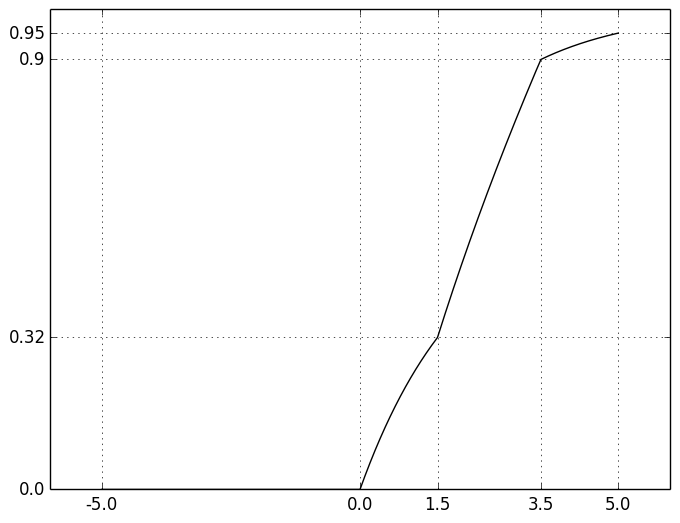
\includegraphics[width=0.8\linewidth]{imgs/mixture_cdf_19.png}


{\pgmlSetup
Identify the component distributions:
\vskip\baselineskip
{\pgmlIndent\let\pgmlItem=\pgmlbulletItem


\pgmlItem{}(3 pts) The exponential component has $\lambda$ of 0.5, the probability of the exponential component assigns to the segment $[0,1.5]$ is \mbox{  \parbox[t]{20ex}{\hrulefill}  }



\pgmlItem{}(3 pts) The weight of the exponential component is \mbox{  \parbox[t]{20ex}{\hrulefill}  }



\pgmlItem{}(2 pts) The weight corresponding to the uniform component is therefore \mbox{  \parbox[t]{20ex}{\hrulefill}  }



\pgmlItem{}(2 pts) The uniform component is over (\mbox{  \parbox[t]{20ex}{\hrulefill}  },\mbox{  \parbox[t]{20ex}{\hrulefill}  }).

\par}%
\par}%
%%%%%%%%%%%%%%%%%%%%%%%%%%%%%%%%%%%%%%%%%%%%%%%%%%%%%%%%%%%%%%%%%%%%%%%%%%%%%%%%
% WeBWorK Online Homework Delivery System
% Copyright � 2000-2007 The WeBWorK Project, http://openwebwork.sf.net/
% $CVSHeader: webwork2/conf/snippets/hardcopyProblemDivider.tex,v 1.3 2004/06/24 21:10:50 dpvc Exp $
% 
% This program is free software; you can redistribute it and/or modify it under
% the terms of either: (a) the GNU General Public License as published by the
% Free Software Foundation; either version 2, or (at your option) any later
% version, or (b) the "Artistic License" which comes with this package.
% 
% This program is distributed in the hope that it will be useful, but WITHOUT
% ANY WARRANTY; without even the implied warranty of MERCHANTABILITY or FITNESS
% FOR A PARTICULAR PURPOSE.  See either the GNU General Public License or the
% Artistic License for more details.
%%%%%%%%%%%%%%%%%%%%%%%%%%%%%%%%%%%%%%%%%%%%%%%%%%%%%%%%%%%%%%%%%%%%%%%%%%%%%%%%


\pagebreak{\bf 6.} (9 pts) \ifdim\lastskip=\pgmlMarker
  \let\pgmlPar=\relax
 \else
  \let\pgmlPar=\par
  \vadjust{\kern3pt}%
\fi

%%%%%%%%%%%%%%%%%%%%%%%%%%%%%%%%%%%%%%
%
%    definitions for PGML
%

\ifx\pgmlCount\undefined  % don not redefine if multiple files load PGML.pl
  \newcount\pgmlCount
  \newdimen\pgmlPercent
  \newdimen\pgmlPixels  \pgmlPixels=.5pt
\fi
\pgmlPercent=.01\hsize

\def\pgmlSetup{%
  \parskip=10pt \parindent=0pt
%  \ifdim\lastskip=\pgmlMarker\else\par\fi
  \pgmlPar
}%

\def\pgmlIndent{\par\advance\leftskip by 2em \advance\pgmlPercent by .02em \pgmlCount=0}%
\def\pgmlbulletItem{\par\indent\llap{$\bullet$ }\ignorespaces}%
\def\pgmlcircleItem{\par\indent\llap{$\circ$ }\ignorespaces}%
\def\pgmlsquareItem{\par\indent\llap{\vrule height 1ex width .75ex depth -.25ex\ }\ignorespaces}%
\def\pgmlnumericItem{\par\indent\advance\pgmlCount by 1 \llap{\the\pgmlCount. }\ignorespaces}%
\def\pgmlalphaItem{\par\indent{\advance\pgmlCount by `\a \llap{\char\pgmlCount. }}\advance\pgmlCount by 1\ignorespaces}%
\def\pgmlAlphaItem{\par\indent{\advance\pgmlCount by `\A \llap{\char\pgmlCount. }}\advance\pgmlCount by 1\ignorespaces}%
\def\pgmlromanItem{\par\indent\advance\pgmlCount by 1 \llap{\romannumeral\pgmlCount. }\ignorespaces}%
\def\pgmlRomanItem{\par\indent\advance\pgmlCount by 1 \llap{\uppercase\expandafter{\romannumeral\pgmlCount}. }\ignorespaces}%

\def\pgmlCenter{%
  \par \parfillskip=0pt
  \advance\leftskip by 0pt plus .5\hsize
  \advance\rightskip by 0pt plus .5\hsize
  \def\pgmlBreak{\break}%
}%
\def\pgmlRight{%
  \par \parfillskip=0pt
  \advance\leftskip by 0pt plus \hsize
  \def\pgmlBreak{\break}%
}%

\def\pgmlBreak{\\}%

\def\pgmlHeading#1{%
  \par\bfseries
  \ifcase#1 \or\huge \or\LARGE \or\large \or\normalsize \or\footnotesize \or\scriptsize \fi
}%

\def\pgmlRule#1#2{%
  \par\noindent
  \hbox{%
    \strut%
    \dimen1=\ht\strutbox%
    \advance\dimen1 by -#2%
    \divide\dimen1 by 2%
    \advance\dimen2 by -\dp\strutbox%
    \raise\dimen1\hbox{\vrule width #1 height #2 depth 0pt}%
  }%
  \par
}%

\def\pgmlIC#1{\futurelet\pgmlNext\pgmlCheckIC}%
\def\pgmlCheckIC{\ifx\pgmlNext\pgmlSpace \/\fi}%
{\def\getSpace#1{\global\let\pgmlSpace= }\getSpace{} }%

{\catcode`\ =12\global\let\pgmlSpaceChar= }%
{\obeylines\gdef\pgmlPreformatted{\par\small\ttfamily\hsize=10\hsize\obeyspaces\obeylines\let^^M=\pgmlNL\pgmlNL}}%
\def\pgmlNL{\par\bgroup\catcode`\ =12\pgmlTestSpace}%
\def\pgmlTestSpace{\futurelet\next\pgmlTestChar}%
\def\pgmlTestChar{\ifx\next\pgmlSpaceChar\ \pgmlTestNext\fi\egroup}%
\def\pgmlTestNext\fi\egroup#1{\fi\pgmlTestSpace}%


%%%%%%%%%%%%%%%%%%%%%%%%%%%%%%%%%%%%%%
{\pgmlSetup
An airline company is considering a new policy of booking as many as 196 persons on an
airplane that can seat only 180.
(Past studies have revealed that only 85\% of the booked passengers actually arrive for the flight.)
\vskip\baselineskip
We want to compute the probability that the number of passengers arriving for the flight is more than 180.
\vskip\baselineskip
Denote by $X_i$ the binary random variable that is 1 if passenger $i$ arrived for the flight and 0 otherwise.
\vskip\baselineskip
Denote by $n$=180  the number passengers that have booked the flight and by $S=\sum_{i=1}^n X_i$ the number of passengers that arrived for the flight. 
\vskip\baselineskip
{\pgmlIndent\let\pgmlItem=\pgmlbulletItem


\pgmlItem{}(3 pts) What is the mean of the number of passengers that arrive for the flight? $E(S)=$ \mbox{  \parbox[t]{20ex}{\hrulefill}  }
\vskip\baselineskip


\pgmlItem{}(3 pts) What is the standard deviation ? $\sqrt{var(S)}=$\mbox{  \parbox[t]{20ex}{\hrulefill}  }
\vskip\baselineskip


\pgmlItem{}(3 pts) Using central-limit theorem and the Q function, estimate the probability that if the company books 196 persons, not enough seats will be 
available.
\par}%
\vskip\baselineskip
\mbox{  \parbox[t]{20ex}{\hrulefill}  }
\par}%
%%%%%%%%%%%%%%%%%%%%%%%%%%%%%%%%%%%%%%%%%%%%%%%%%%%%%%%%%%%%%%%%%%%%%%%%%%%%%%%%
% WeBWorK Online Homework Delivery System
% Copyright � 2000-2007 The WeBWorK Project, http://openwebwork.sf.net/
% $CVSHeader: webwork2/conf/snippets/hardcopyProblemDivider.tex,v 1.3 2004/06/24 21:10:50 dpvc Exp $
% 
% This program is free software; you can redistribute it and/or modify it under
% the terms of either: (a) the GNU General Public License as published by the
% Free Software Foundation; either version 2, or (at your option) any later
% version, or (b) the "Artistic License" which comes with this package.
% 
% This program is distributed in the hope that it will be useful, but WITHOUT
% ANY WARRANTY; without even the implied warranty of MERCHANTABILITY or FITNESS
% FOR A PARTICULAR PURPOSE.  See either the GNU General Public License or the
% Artistic License for more details.
%%%%%%%%%%%%%%%%%%%%%%%%%%%%%%%%%%%%%%%%%%%%%%%%%%%%%%%%%%%%%%%%%%%%%%%%%%%%%%%%


\pagebreak{\bf 7.} (9 pts) \ifdim\lastskip=\pgmlMarker
  \let\pgmlPar=\relax
 \else
  \let\pgmlPar=\par
  \vadjust{\kern3pt}%
\fi

%%%%%%%%%%%%%%%%%%%%%%%%%%%%%%%%%%%%%%
%
%    definitions for PGML
%

\ifx\pgmlCount\undefined  % don not redefine if multiple files load PGML.pl
  \newcount\pgmlCount
  \newdimen\pgmlPercent
  \newdimen\pgmlPixels  \pgmlPixels=.5pt
\fi
\pgmlPercent=.01\hsize

\def\pgmlSetup{%
  \parskip=10pt \parindent=0pt
%  \ifdim\lastskip=\pgmlMarker\else\par\fi
  \pgmlPar
}%

\def\pgmlIndent{\par\advance\leftskip by 2em \advance\pgmlPercent by .02em \pgmlCount=0}%
\def\pgmlbulletItem{\par\indent\llap{$\bullet$ }\ignorespaces}%
\def\pgmlcircleItem{\par\indent\llap{$\circ$ }\ignorespaces}%
\def\pgmlsquareItem{\par\indent\llap{\vrule height 1ex width .75ex depth -.25ex\ }\ignorespaces}%
\def\pgmlnumericItem{\par\indent\advance\pgmlCount by 1 \llap{\the\pgmlCount. }\ignorespaces}%
\def\pgmlalphaItem{\par\indent{\advance\pgmlCount by `\a \llap{\char\pgmlCount. }}\advance\pgmlCount by 1\ignorespaces}%
\def\pgmlAlphaItem{\par\indent{\advance\pgmlCount by `\A \llap{\char\pgmlCount. }}\advance\pgmlCount by 1\ignorespaces}%
\def\pgmlromanItem{\par\indent\advance\pgmlCount by 1 \llap{\romannumeral\pgmlCount. }\ignorespaces}%
\def\pgmlRomanItem{\par\indent\advance\pgmlCount by 1 \llap{\uppercase\expandafter{\romannumeral\pgmlCount}. }\ignorespaces}%

\def\pgmlCenter{%
  \par \parfillskip=0pt
  \advance\leftskip by 0pt plus .5\hsize
  \advance\rightskip by 0pt plus .5\hsize
  \def\pgmlBreak{\break}%
}%
\def\pgmlRight{%
  \par \parfillskip=0pt
  \advance\leftskip by 0pt plus \hsize
  \def\pgmlBreak{\break}%
}%

\def\pgmlBreak{\\}%

\def\pgmlHeading#1{%
  \par\bfseries
  \ifcase#1 \or\huge \or\LARGE \or\large \or\normalsize \or\footnotesize \or\scriptsize \fi
}%

\def\pgmlRule#1#2{%
  \par\noindent
  \hbox{%
    \strut%
    \dimen1=\ht\strutbox%
    \advance\dimen1 by -#2%
    \divide\dimen1 by 2%
    \advance\dimen2 by -\dp\strutbox%
    \raise\dimen1\hbox{\vrule width #1 height #2 depth 0pt}%
  }%
  \par
}%

\def\pgmlIC#1{\futurelet\pgmlNext\pgmlCheckIC}%
\def\pgmlCheckIC{\ifx\pgmlNext\pgmlSpace \/\fi}%
{\def\getSpace#1{\global\let\pgmlSpace= }\getSpace{} }%

{\catcode`\ =12\global\let\pgmlSpaceChar= }%
{\obeylines\gdef\pgmlPreformatted{\par\small\ttfamily\hsize=10\hsize\obeyspaces\obeylines\let^^M=\pgmlNL\pgmlNL}}%
\def\pgmlNL{\par\bgroup\catcode`\ =12\pgmlTestSpace}%
\def\pgmlTestSpace{\futurelet\next\pgmlTestChar}%
\def\pgmlTestChar{\ifx\next\pgmlSpaceChar\ \pgmlTestNext\fi\egroup}%
\def\pgmlTestNext\fi\egroup#1{\fi\pgmlTestSpace}%


%%%%%%%%%%%%%%%%%%%%%%%%%%%%%%%%%%%%%%
{\pgmlSetup
Let $X$ be a number that is uniformly distributed in $U$(38, 98). Let $S$ be the average of n = 48 samples of $X$: $S = \frac{1}{n} \sum_{i=1}^{n}X_i$.
{\pgmlIndent\let\pgmlItem=\pgmlnumericItem


\pgmlItem{}(3 pts) $\mathbb{E}(S) = $\mbox{  \parbox[t]{20ex}{\hrulefill}  }



\pgmlItem{}(3 pts) $Var(S) = $\mbox{  \parbox[t]{20ex}{\hrulefill}  }
{\bfseries{}Hint: }The formular for the variance of the $U$(a, b) is $\frac{(b-a)^2}{12}$



\pgmlItem{}(3 pts) Using Q function in your answer, what is the approximate probability of $P(S > 90)$\mbox{  \parbox[t]{20ex}{\hrulefill}  }

\par}%
\par}%
%%%%%%%%%%%%%%%%%%%%%%%%%%%%%%%%%%%%%%%%%%%%%%%%%%%%%%%%%%%%%%%%%%%%%%%%%%%%%%%%
% WeBWorK Online Homework Delivery System
% Copyright � 2000-2007 The WeBWorK Project, http://openwebwork.sf.net/
% $CVSHeader: webwork2/conf/snippets/hardcopyProblemDivider.tex,v 1.3 2004/06/24 21:10:50 dpvc Exp $
% 
% This program is free software; you can redistribute it and/or modify it under
% the terms of either: (a) the GNU General Public License as published by the
% Free Software Foundation; either version 2, or (at your option) any later
% version, or (b) the "Artistic License" which comes with this package.
% 
% This program is distributed in the hope that it will be useful, but WITHOUT
% ANY WARRANTY; without even the implied warranty of MERCHANTABILITY or FITNESS
% FOR A PARTICULAR PURPOSE.  See either the GNU General Public License or the
% Artistic License for more details.
%%%%%%%%%%%%%%%%%%%%%%%%%%%%%%%%%%%%%%%%%%%%%%%%%%%%%%%%%%%%%%%%%%%%%%%%%%%%%%%%



      \ifx\pgmlMarker\undefined
        \newdimen\pgmlMarker \pgmlMarker=0.00314159pt  % hack to lett if \newline was used
      \fi
      \ifx\oldnewline\undefined \let\oldnewline=\newline \fi
      \def\newline{\oldnewline\hskip-\pgmlMarker\hskip\pgmlMarker\relax}%
      \parindent=0pt
      \catcode`\^^M=\active
      \def^^M{\ifmmode\else\fi\ignorespaces}%  skip paragraph breaks in the preamble
      \def\par{\ifmmode\else\endgraf\fi\ignorespaces}%
    \pagebreak{\bf 8.} (9 pts) \ifdim\lastskip=\pgmlMarker
  \let\pgmlPar=\relax
 \else
  \let\pgmlPar=\par
  \vadjust{\kern3pt}%
\fi

%%%%%%%%%%%%%%%%%%%%%%%%%%%%%%%%%%%%%%
%
%    definitions for PGML
%

\ifx\pgmlCount\undefined  % don not redefine if multiple files load PGML.pl
  \newcount\pgmlCount
  \newdimen\pgmlPercent
  \newdimen\pgmlPixels  \pgmlPixels=.5pt
\fi
\pgmlPercent=.01\hsize

\def\pgmlSetup{%
  \parskip=10pt \parindent=0pt
%  \ifdim\lastskip=\pgmlMarker\else\par\fi
  \pgmlPar
}%

\def\pgmlIndent{\par\advance\leftskip by 2em \advance\pgmlPercent by .02em \pgmlCount=0}%
\def\pgmlbulletItem{\par\indent\llap{$\bullet$ }\ignorespaces}%
\def\pgmlcircleItem{\par\indent\llap{$\circ$ }\ignorespaces}%
\def\pgmlsquareItem{\par\indent\llap{\vrule height 1ex width .75ex depth -.25ex\ }\ignorespaces}%
\def\pgmlnumericItem{\par\indent\advance\pgmlCount by 1 \llap{\the\pgmlCount. }\ignorespaces}%
\def\pgmlalphaItem{\par\indent{\advance\pgmlCount by `\a \llap{\char\pgmlCount. }}\advance\pgmlCount by 1\ignorespaces}%
\def\pgmlAlphaItem{\par\indent{\advance\pgmlCount by `\A \llap{\char\pgmlCount. }}\advance\pgmlCount by 1\ignorespaces}%
\def\pgmlromanItem{\par\indent\advance\pgmlCount by 1 \llap{\romannumeral\pgmlCount. }\ignorespaces}%
\def\pgmlRomanItem{\par\indent\advance\pgmlCount by 1 \llap{\uppercase\expandafter{\romannumeral\pgmlCount}. }\ignorespaces}%

\def\pgmlCenter{%
  \par \parfillskip=0pt
  \advance\leftskip by 0pt plus .5\hsize
  \advance\rightskip by 0pt plus .5\hsize
  \def\pgmlBreak{\break}%
}%
\def\pgmlRight{%
  \par \parfillskip=0pt
  \advance\leftskip by 0pt plus \hsize
  \def\pgmlBreak{\break}%
}%

\def\pgmlBreak{\\}%

\def\pgmlHeading#1{%
  \par\bfseries
  \ifcase#1 \or\huge \or\LARGE \or\large \or\normalsize \or\footnotesize \or\scriptsize \fi
}%

\def\pgmlRule#1#2{%
  \par\noindent
  \hbox{%
    \strut%
    \dimen1=\ht\strutbox%
    \advance\dimen1 by -#2%
    \divide\dimen1 by 2%
    \advance\dimen2 by -\dp\strutbox%
    \raise\dimen1\hbox{\vrule width #1 height #2 depth 0pt}%
  }%
  \par
}%

\def\pgmlIC#1{\futurelet\pgmlNext\pgmlCheckIC}%
\def\pgmlCheckIC{\ifx\pgmlNext\pgmlSpace \/\fi}%
{\def\getSpace#1{\global\let\pgmlSpace= }\getSpace{} }%

{\catcode`\ =12\global\let\pgmlSpaceChar= }%
{\obeylines\gdef\pgmlPreformatted{\par\small\ttfamily\hsize=10\hsize\obeyspaces\obeylines\let^^M=\pgmlNL\pgmlNL}}%
\def\pgmlNL{\par\bgroup\catcode`\ =12\pgmlTestSpace}%
\def\pgmlTestSpace{\futurelet\next\pgmlTestChar}%
\def\pgmlTestChar{\ifx\next\pgmlSpaceChar\ \pgmlTestNext\fi\egroup}%
\def\pgmlTestNext\fi\egroup#1{\fi\pgmlTestSpace}%


%%%%%%%%%%%%%%%%%%%%%%%%%%%%%%%%%%%%%%
{\pgmlSetup
Suppose $X_1, ... , X_{56}$ are IID random variables where $X_i \in \{0,1\}$ and $P(X_i = 1) = 0.3$ for $i = 1, ..., n$.
\vskip\baselineskip
Define a random variable $Y = \sum_{i=1}^{56}{(-1)^{i+1} X_i} = X_1 - X_2 + X_3 - X_4 + ... - X_{56}$
\vskip\baselineskip
(3 pts) What is $E[Y]$?  \mbox{  \parbox[t]{20ex}{\hrulefill}  }
\vskip\baselineskip
(3 pts) What is $Var[Y]$?  \mbox{  \parbox[t]{20ex}{\hrulefill}  }
\vskip\baselineskip
(3 pts) Using Chebyshev's inequality, give an upper bound on $P(|Y| > 26)$?  \mbox{  \parbox[t]{20ex}{\hrulefill}  }
\par}%
%%%%%%%%%%%%%%%%%%%%%%%%%%%%%%%%%%%%%%%%%%%%%%%%%%%%%%%%%%%%%%%%%%%%%%%%%%%%%%%%
% WeBWorK Online Homework Delivery System
% Copyright � 2000-2007 The WeBWorK Project, http://openwebwork.sf.net/
% $CVSHeader: webwork2/conf/snippets/hardcopyProblemDivider.tex,v 1.3 2004/06/24 21:10:50 dpvc Exp $
% 
% This program is free software; you can redistribute it and/or modify it under
% the terms of either: (a) the GNU General Public License as published by the
% Free Software Foundation; either version 2, or (at your option) any later
% version, or (b) the "Artistic License" which comes with this package.
% 
% This program is distributed in the hope that it will be useful, but WITHOUT
% ANY WARRANTY; without even the implied warranty of MERCHANTABILITY or FITNESS
% FOR A PARTICULAR PURPOSE.  See either the GNU General Public License or the
% Artistic License for more details.
%%%%%%%%%%%%%%%%%%%%%%%%%%%%%%%%%%%%%%%%%%%%%%%%%%%%%%%%%%%%%%%%%%%%%%%%%%%%%%%%



      \ifx\pgmlMarker\undefined
        \newdimen\pgmlMarker \pgmlMarker=0.00314159pt  % hack to lett if \newline was used
      \fi
      \ifx\oldnewline\undefined \let\oldnewline=\newline \fi
      \def\newline{\oldnewline\hskip-\pgmlMarker\hskip\pgmlMarker\relax}%
      \parindent=0pt
      \catcode`\^^M=\active
      \def^^M{\ifmmode\else\fi\ignorespaces}%  skip paragraph breaks in the preamble
      \def\par{\ifmmode\else\endgraf\fi\ignorespaces}%
    \pagebreak{\bf 9.} (20 pts) \ifdim\lastskip=\pgmlMarker
  \let\pgmlPar=\relax
 \else
  \let\pgmlPar=\par
  \vadjust{\kern3pt}%
\fi

%%%%%%%%%%%%%%%%%%%%%%%%%%%%%%%%%%%%%%
%
%    definitions for PGML
%

\ifx\pgmlCount\undefined  % don not redefine if multiple files load PGML.pl
  \newcount\pgmlCount
  \newdimen\pgmlPercent
  \newdimen\pgmlPixels  \pgmlPixels=.5pt
\fi
\pgmlPercent=.01\hsize

\def\pgmlSetup{%
  \parskip=10pt \parindent=0pt
%  \ifdim\lastskip=\pgmlMarker\else\par\fi
  \pgmlPar
}%

\def\pgmlIndent{\par\advance\leftskip by 2em \advance\pgmlPercent by .02em \pgmlCount=0}%
\def\pgmlbulletItem{\par\indent\llap{$\bullet$ }\ignorespaces}%
\def\pgmlcircleItem{\par\indent\llap{$\circ$ }\ignorespaces}%
\def\pgmlsquareItem{\par\indent\llap{\vrule height 1ex width .75ex depth -.25ex\ }\ignorespaces}%
\def\pgmlnumericItem{\par\indent\advance\pgmlCount by 1 \llap{\the\pgmlCount. }\ignorespaces}%
\def\pgmlalphaItem{\par\indent{\advance\pgmlCount by `\a \llap{\char\pgmlCount. }}\advance\pgmlCount by 1\ignorespaces}%
\def\pgmlAlphaItem{\par\indent{\advance\pgmlCount by `\A \llap{\char\pgmlCount. }}\advance\pgmlCount by 1\ignorespaces}%
\def\pgmlromanItem{\par\indent\advance\pgmlCount by 1 \llap{\romannumeral\pgmlCount. }\ignorespaces}%
\def\pgmlRomanItem{\par\indent\advance\pgmlCount by 1 \llap{\uppercase\expandafter{\romannumeral\pgmlCount}. }\ignorespaces}%

\def\pgmlCenter{%
  \par \parfillskip=0pt
  \advance\leftskip by 0pt plus .5\hsize
  \advance\rightskip by 0pt plus .5\hsize
  \def\pgmlBreak{\break}%
}%
\def\pgmlRight{%
  \par \parfillskip=0pt
  \advance\leftskip by 0pt plus \hsize
  \def\pgmlBreak{\break}%
}%

\def\pgmlBreak{\\}%

\def\pgmlHeading#1{%
  \par\bfseries
  \ifcase#1 \or\huge \or\LARGE \or\large \or\normalsize \or\footnotesize \or\scriptsize \fi
}%

\def\pgmlRule#1#2{%
  \par\noindent
  \hbox{%
    \strut%
    \dimen1=\ht\strutbox%
    \advance\dimen1 by -#2%
    \divide\dimen1 by 2%
    \advance\dimen2 by -\dp\strutbox%
    \raise\dimen1\hbox{\vrule width #1 height #2 depth 0pt}%
  }%
  \par
}%

\def\pgmlIC#1{\futurelet\pgmlNext\pgmlCheckIC}%
\def\pgmlCheckIC{\ifx\pgmlNext\pgmlSpace \/\fi}%
{\def\getSpace#1{\global\let\pgmlSpace= }\getSpace{} }%

{\catcode`\ =12\global\let\pgmlSpaceChar= }%
{\obeylines\gdef\pgmlPreformatted{\par\small\ttfamily\hsize=10\hsize\obeyspaces\obeylines\let^^M=\pgmlNL\pgmlNL}}%
\def\pgmlNL{\par\bgroup\catcode`\ =12\pgmlTestSpace}%
\def\pgmlTestSpace{\futurelet\next\pgmlTestChar}%
\def\pgmlTestChar{\ifx\next\pgmlSpaceChar\ \pgmlTestNext\fi\egroup}%
\def\pgmlTestNext\fi\egroup#1{\fi\pgmlTestSpace}%


%%%%%%%%%%%%%%%%%%%%%%%%%%%%%%%%%%%%%%
{\pgmlSetup
Let $X_1,X_2,X_3,X_4$ be IID binary random variables for which $P(X_i=-1)=P(X_i=+1)=1/2$.

{\pgmlIndent\let\pgmlItem=\pgmlbulletItem


\pgmlItem{}Define $Y_1=X_1+X_2$ and $Y_2=X_3+X_4$.
\vskip\baselineskip
(1 pt) Are $Y_1,Y_2$ independent (yes/no)? \mbox{  \parbox[t]{20ex}{\hrulefill}  }
\vskip\baselineskip
(2 pts) For any $i \in \{1,2,3,4\}$, the expectation $E(Y_i)$=\mbox{  \parbox[t]{20ex}{\hrulefill}  }.
\vskip\baselineskip
Recall that for any two random variables $A,B$, the covariance is defined as $Cov(A,B) = E(AB) - E(A)E(B)$.
\vskip\baselineskip
(2 pts) For any $i \in \{1,2,3,4\}$, $E(X_i^2)$=\mbox{  \parbox[t]{20ex}{\hrulefill}  }.
\vskip\baselineskip
(2 pts) For any $i \neq j$, $E(X_i X_j)$=\mbox{  \parbox[t]{20ex}{\hrulefill}  }.
\vskip\baselineskip
(3 pts) $Cov(Y_1,Y_2)$=\mbox{  \parbox[t]{20ex}{\hrulefill}  }
\par}%
\vskip\baselineskip

\vskip\baselineskip
{\pgmlIndent\let\pgmlItem=\pgmlbulletItem


\pgmlItem{}Define $Y_3=X_2+X_3$.
\vskip\baselineskip
(1 pt) Are $Y_1,Y_3$ independent (yes/no)? \mbox{  \parbox[t]{20ex}{\hrulefill}  }
\vskip\baselineskip
(1 pt) Are $Y_2,Y_3$ independent (yes/no)? \mbox{  \parbox[t]{20ex}{\hrulefill}  }
\vskip\baselineskip
(2 pts) $Cov(Y_1,Y_3)$=\mbox{  \parbox[t]{20ex}{\hrulefill}  }.
\par}%
\vskip\baselineskip

\vskip\baselineskip
{\pgmlIndent\let\pgmlItem=\pgmlbulletItem


\pgmlItem{}Recall the definition of the correlation coefficient:
$Corr(A,B) = \frac{Cov(A,B)}{\sqrt{var(A) var(B)}}$.
\vskip\baselineskip
(2 pts) For any $i \in \{1,2,3\}$, $var(Y_i)$=\mbox{  \parbox[t]{20ex}{\hrulefill}  }.
\vskip\baselineskip
(2 pts) $Corr(Y_1,Y_2)$=\mbox{  \parbox[t]{20ex}{\hrulefill}  }.
\vskip\baselineskip
(2 pts) $Corr(Y_1,Y_3)$=\mbox{  \parbox[t]{20ex}{\hrulefill}  }.

\par}%
\par}%
%%%%%%%%%%%%%%%%%%%%%%%%%%%%%%%%%%%%%%%%%%%%%%%%%%%%%%%%%%%%%%%%%%%%%%%%%%%%%%%%
% WeBWorK Online Homework Delivery System
% Copyright � 2000-2007 The WeBWorK Project, http://openwebwork.sf.net/
% $CVSHeader: webwork2/conf/snippets/hardcopyProblemDivider.tex,v 1.3 2004/06/24 21:10:50 dpvc Exp $
% 
% This program is free software; you can redistribute it and/or modify it under
% the terms of either: (a) the GNU General Public License as published by the
% Free Software Foundation; either version 2, or (at your option) any later
% version, or (b) the "Artistic License" which comes with this package.
% 
% This program is distributed in the hope that it will be useful, but WITHOUT
% ANY WARRANTY; without even the implied warranty of MERCHANTABILITY or FITNESS
% FOR A PARTICULAR PURPOSE.  See either the GNU General Public License or the
% Artistic License for more details.
%%%%%%%%%%%%%%%%%%%%%%%%%%%%%%%%%%%%%%%%%%%%%%%%%%%%%%%%%%%%%%%%%%%%%%%%%%%%%%%%



      \ifx\pgmlMarker\undefined
        \newdimen\pgmlMarker \pgmlMarker=0.00314159pt  % hack to lett if \newline was used
      \fi
      \ifx\oldnewline\undefined \let\oldnewline=\newline \fi
      \def\newline{\oldnewline\hskip-\pgmlMarker\hskip\pgmlMarker\relax}%
      \parindent=0pt
      \catcode`\^^M=\active
      \def^^M{\ifmmode\else\fi\ignorespaces}%  skip paragraph breaks in the preamble
      \def\par{\ifmmode\else\endgraf\fi\ignorespaces}%
    \pagebreak{\bf 10.} (11 pts) \ifdim\lastskip=\pgmlMarker
  \let\pgmlPar=\relax
 \else
  \let\pgmlPar=\par
  \vadjust{\kern3pt}%
\fi

%%%%%%%%%%%%%%%%%%%%%%%%%%%%%%%%%%%%%%
%
%    definitions for PGML
%

\ifx\pgmlCount\undefined  % don not redefine if multiple files load PGML.pl
  \newcount\pgmlCount
  \newdimen\pgmlPercent
  \newdimen\pgmlPixels  \pgmlPixels=.5pt
\fi
\pgmlPercent=.01\hsize

\def\pgmlSetup{%
  \parskip=10pt \parindent=0pt
%  \ifdim\lastskip=\pgmlMarker\else\par\fi
  \pgmlPar
}%

\def\pgmlIndent{\par\advance\leftskip by 2em \advance\pgmlPercent by .02em \pgmlCount=0}%
\def\pgmlbulletItem{\par\indent\llap{$\bullet$ }\ignorespaces}%
\def\pgmlcircleItem{\par\indent\llap{$\circ$ }\ignorespaces}%
\def\pgmlsquareItem{\par\indent\llap{\vrule height 1ex width .75ex depth -.25ex\ }\ignorespaces}%
\def\pgmlnumericItem{\par\indent\advance\pgmlCount by 1 \llap{\the\pgmlCount. }\ignorespaces}%
\def\pgmlalphaItem{\par\indent{\advance\pgmlCount by `\a \llap{\char\pgmlCount. }}\advance\pgmlCount by 1\ignorespaces}%
\def\pgmlAlphaItem{\par\indent{\advance\pgmlCount by `\A \llap{\char\pgmlCount. }}\advance\pgmlCount by 1\ignorespaces}%
\def\pgmlromanItem{\par\indent\advance\pgmlCount by 1 \llap{\romannumeral\pgmlCount. }\ignorespaces}%
\def\pgmlRomanItem{\par\indent\advance\pgmlCount by 1 \llap{\uppercase\expandafter{\romannumeral\pgmlCount}. }\ignorespaces}%

\def\pgmlCenter{%
  \par \parfillskip=0pt
  \advance\leftskip by 0pt plus .5\hsize
  \advance\rightskip by 0pt plus .5\hsize
  \def\pgmlBreak{\break}%
}%
\def\pgmlRight{%
  \par \parfillskip=0pt
  \advance\leftskip by 0pt plus \hsize
  \def\pgmlBreak{\break}%
}%

\def\pgmlBreak{\\}%

\def\pgmlHeading#1{%
  \par\bfseries
  \ifcase#1 \or\huge \or\LARGE \or\large \or\normalsize \or\footnotesize \or\scriptsize \fi
}%

\def\pgmlRule#1#2{%
  \par\noindent
  \hbox{%
    \strut%
    \dimen1=\ht\strutbox%
    \advance\dimen1 by -#2%
    \divide\dimen1 by 2%
    \advance\dimen2 by -\dp\strutbox%
    \raise\dimen1\hbox{\vrule width #1 height #2 depth 0pt}%
  }%
  \par
}%

\def\pgmlIC#1{\futurelet\pgmlNext\pgmlCheckIC}%
\def\pgmlCheckIC{\ifx\pgmlNext\pgmlSpace \/\fi}%
{\def\getSpace#1{\global\let\pgmlSpace= }\getSpace{} }%

{\catcode`\ =12\global\let\pgmlSpaceChar= }%
{\obeylines\gdef\pgmlPreformatted{\par\small\ttfamily\hsize=10\hsize\obeyspaces\obeylines\let^^M=\pgmlNL\pgmlNL}}%
\def\pgmlNL{\par\bgroup\catcode`\ =12\pgmlTestSpace}%
\def\pgmlTestSpace{\futurelet\next\pgmlTestChar}%
\def\pgmlTestChar{\ifx\next\pgmlSpaceChar\ \pgmlTestNext\fi\egroup}%
\def\pgmlTestNext\fi\egroup#1{\fi\pgmlTestSpace}%


%%%%%%%%%%%%%%%%%%%%%%%%%%%%%%%%%%%%%%
{\pgmlSetup
Suppose you have a web server, with HTTP request packets arriving independently at random. The expected time between requests is 0.01.
\vskip\baselineskip
(2 pts) What is the expected number of packets that arrive per second? \mbox{  \parbox[t]{20ex}{\hrulefill}  }
\vskip\baselineskip
(3 pts) What is the probability that over 200 packets will arrive during a particular second? \mbox{  \parbox[t]{20ex}{\hrulefill}  }
\vskip\baselineskip
(3 pts) Consider an hour as a sequence of one second bins (i.e. 3600 1-second bins). What is the expected number of bins during which more than 200 packets will arrive?
\vskip\baselineskip
\mbox{  \parbox[t]{20ex}{\hrulefill}  }
\vskip\baselineskip
(3 pts) What is the probability that the time gap between two packets is larger than 0.025? \mbox{  \parbox[t]{20ex}{\hrulefill}  }
\vskip\baselineskip
{\bfseries{}Note1:} In one of the answers above you might need to use an infinite sum.
\vskip\baselineskip
{\bfseries{}Note2:} You may find the following formulas useful:
\vskip\baselineskip
Poisson PDF: $P(X=k) = \frac{\lambda^k}{k!} e^{-\lambda}$
\vskip\baselineskip
Exponential PDF: $P(X=k) = \lambda e^{-\lambda k}$
\vskip\baselineskip
Exponential CDF: $P(X \le k) = 1- e^{-\lambda k}$
\par}%
%%%%%%%%%%%%%%%%%%%%%%%%%%%%%%%%%%%%%%%%%%%%%%%%%%%%%%%%%%%%%%%%%%%%%%%%%%%%%%%%
% WeBWorK Online Homework Delivery System
% Copyright � 2000-2007 The WeBWorK Project, http://openwebwork.sf.net/
% $CVSHeader: webwork2/conf/snippets/hardcopyProblemDivider.tex,v 1.3 2004/06/24 21:10:50 dpvc Exp $
% 
% This program is free software; you can redistribute it and/or modify it under
% the terms of either: (a) the GNU General Public License as published by the
% Free Software Foundation; either version 2, or (at your option) any later
% version, or (b) the "Artistic License" which comes with this package.
% 
% This program is distributed in the hope that it will be useful, but WITHOUT
% ANY WARRANTY; without even the implied warranty of MERCHANTABILITY or FITNESS
% FOR A PARTICULAR PURPOSE.  See either the GNU General Public License or the
% Artistic License for more details.
%%%%%%%%%%%%%%%%%%%%%%%%%%%%%%%%%%%%%%%%%%%%%%%%%%%%%%%%%%%%%%%%%%%%%%%%%%%%%%%%


\pagebreak{\bf 11.} (16 pts) \ifdim\lastskip=\pgmlMarker
  \let\pgmlPar=\relax
 \else
  \let\pgmlPar=\par
  \vadjust{\kern3pt}%
\fi

%%%%%%%%%%%%%%%%%%%%%%%%%%%%%%%%%%%%%%
%
%    definitions for PGML
%

\ifx\pgmlCount\undefined  % don not redefine if multiple files load PGML.pl
  \newcount\pgmlCount
  \newdimen\pgmlPercent
  \newdimen\pgmlPixels  \pgmlPixels=.5pt
\fi
\pgmlPercent=.01\hsize

\def\pgmlSetup{%
  \parskip=10pt \parindent=0pt
%  \ifdim\lastskip=\pgmlMarker\else\par\fi
  \pgmlPar
}%

\def\pgmlIndent{\par\advance\leftskip by 2em \advance\pgmlPercent by .02em \pgmlCount=0}%
\def\pgmlbulletItem{\par\indent\llap{$\bullet$ }\ignorespaces}%
\def\pgmlcircleItem{\par\indent\llap{$\circ$ }\ignorespaces}%
\def\pgmlsquareItem{\par\indent\llap{\vrule height 1ex width .75ex depth -.25ex\ }\ignorespaces}%
\def\pgmlnumericItem{\par\indent\advance\pgmlCount by 1 \llap{\the\pgmlCount. }\ignorespaces}%
\def\pgmlalphaItem{\par\indent{\advance\pgmlCount by `\a \llap{\char\pgmlCount. }}\advance\pgmlCount by 1\ignorespaces}%
\def\pgmlAlphaItem{\par\indent{\advance\pgmlCount by `\A \llap{\char\pgmlCount. }}\advance\pgmlCount by 1\ignorespaces}%
\def\pgmlromanItem{\par\indent\advance\pgmlCount by 1 \llap{\romannumeral\pgmlCount. }\ignorespaces}%
\def\pgmlRomanItem{\par\indent\advance\pgmlCount by 1 \llap{\uppercase\expandafter{\romannumeral\pgmlCount}. }\ignorespaces}%

\def\pgmlCenter{%
  \par \parfillskip=0pt
  \advance\leftskip by 0pt plus .5\hsize
  \advance\rightskip by 0pt plus .5\hsize
  \def\pgmlBreak{\break}%
}%
\def\pgmlRight{%
  \par \parfillskip=0pt
  \advance\leftskip by 0pt plus \hsize
  \def\pgmlBreak{\break}%
}%

\def\pgmlBreak{\\}%

\def\pgmlHeading#1{%
  \par\bfseries
  \ifcase#1 \or\huge \or\LARGE \or\large \or\normalsize \or\footnotesize \or\scriptsize \fi
}%

\def\pgmlRule#1#2{%
  \par\noindent
  \hbox{%
    \strut%
    \dimen1=\ht\strutbox%
    \advance\dimen1 by -#2%
    \divide\dimen1 by 2%
    \advance\dimen2 by -\dp\strutbox%
    \raise\dimen1\hbox{\vrule width #1 height #2 depth 0pt}%
  }%
  \par
}%

\def\pgmlIC#1{\futurelet\pgmlNext\pgmlCheckIC}%
\def\pgmlCheckIC{\ifx\pgmlNext\pgmlSpace \/\fi}%
{\def\getSpace#1{\global\let\pgmlSpace= }\getSpace{} }%

{\catcode`\ =12\global\let\pgmlSpaceChar= }%
{\obeylines\gdef\pgmlPreformatted{\par\small\ttfamily\hsize=10\hsize\obeyspaces\obeylines\let^^M=\pgmlNL\pgmlNL}}%
\def\pgmlNL{\par\bgroup\catcode`\ =12\pgmlTestSpace}%
\def\pgmlTestSpace{\futurelet\next\pgmlTestChar}%
\def\pgmlTestChar{\ifx\next\pgmlSpaceChar\ \pgmlTestNext\fi\egroup}%
\def\pgmlTestNext\fi\egroup#1{\fi\pgmlTestSpace}%


%%%%%%%%%%%%%%%%%%%%%%%%%%%%%%%%%%%%%%
{\pgmlSetup
You have an algorithm A for testing whether a Boolean formula f is satisfiable or not, but it is only correct with probability $4/5$. More precisely, you can repeatedly run A on the same formula f, and each time it outputs the correct answer with probability $4/5$.
\vskip\baselineskip
To reduce the probability of error, you run A(f) $n$ times, and return the majority answer. What should $n$ be if you want the probability of error to be less than 0.05?
\vskip\baselineskip

\vskip\baselineskip
Let $C_i$ be a binary random variable indicating whether the $i^{th}$ execution of algorithm A is correct.  Let $C = (C_1 + C_2 ... C_n)/n$.
{\pgmlIndent\let\pgmlItem=\pgmlbulletItem


\pgmlItem{}(2 pts) What is the minimum value of $C$ such that our method of returning the majority answer will be correct?  \mbox{  \parbox[t]{20ex}{\hrulefill}  }



\pgmlItem{}(2 pts) What is $\mathbb{E}(C)$?  \mbox{  \parbox[t]{20ex}{\hrulefill}  }



\pgmlItem{}(2 pts) What is $var(C)$?  \mbox{  \parbox[t]{20ex}{\hrulefill}  } (Use $n$ as variable in this answer)
\par}%
\vskip\baselineskip

{\itshape{}Approach 1}:
Chebyshev's inequality says for random variable $Y$ with mean $\mu$ and for any positive number $a>0$, $P(|Y-\mu| \geq a) \leq var(Y)/a^2$
{\pgmlIndent\let\pgmlItem=\pgmlbulletItem


\pgmlItem{}(3 pts) Using Chebyshev's inequality, what is an upper bound on the probability your ``majority algorithm'' is incorrect?
\par}%
\vskip\baselineskip
\mbox{  \parbox[t]{20ex}{\hrulefill}  }  (Use $n$ as variable in this answer)
\vskip\baselineskip
{\pgmlIndent\let\pgmlItem=\pgmlbulletItem


\pgmlItem{}(2 pts) What is the lower bound on $n$ so that the probability that the ``majority algorithm'' makes an error is  at most 0.05?
\par}%
\vskip\baselineskip
\mbox{  \parbox[t]{20ex}{\hrulefill}  }
\vskip\baselineskip

\vskip\baselineskip
{\itshape{}Approach 2}:
Using Central Limit Theorem, approximate the distribution of $C$ as a normal. 
{\pgmlIndent\let\pgmlItem=\pgmlbulletItem


\pgmlItem{}(3 pts) What is the z-score of $C=0.5$ \mbox{  \parbox[t]{20ex}{\hrulefill}  } (Use $n$ as variable in this answer)



\pgmlItem{}(2 pts) What is the lower bound on $n$ so that the ``majority algorithm'' makes an error with probability at most 0.05? \mbox{  \parbox[t]{20ex}{\hrulefill}  } (Use Q function in your answer)

\par}%
\par}%



\columnwidth=\linewidth


%%%%%%%%%%%%%%%%%%%%%%%%%%%%%%%%%%%%%%%%%%%%%%%%%%%%%%%%%%%%%%%%%%%%%%%%%%%%%%%%
% WeBWorK Online Homework Delivery System
% Copyright � 2000-2007 The WeBWorK Project, http://openwebwork.sf.net/
% $CVSHeader: webwork2/conf/snippets/hardcopyPostamble.tex,v 1.2 2003/12/09 01:12:29 sh002i Exp $
% 
% This program is free software; you can redistribute it and/or modify it under
% the terms of either: (a) the GNU General Public License as published by the
% Free Software Foundation; either version 2, or (at your option) any later
% version, or (b) the "Artistic License" which comes with this package.
% 
% This program is distributed in the hope that it will be useful, but WITHOUT
% ANY WARRANTY; without even the implied warranty of MERCHANTABILITY or FITNESS
% FOR A PARTICULAR PURPOSE.  See either the GNU General Public License or the
% Artistic License for more details.
%%%%%%%%%%%%%%%%%%%%%%%%%%%%%%%%%%%%%%%%%%%%%%%%%%%%%%%%%%%%%%%%%%%%%%%%%%%%%%%%
\vfill
\end{document}

